\documentclass[10pt]{article}

\usepackage[margin=1in]{geometry}
\usepackage[pdftex]{graphicx}
\usepackage[
backend=biber,
style=numeric,
]{biblatex}
\usepackage[shortlabels]{enumitem}
\usepackage{float}
\usepackage{fancyhdr}
\usepackage{parskip}
\usepackage{xcolor}
\usepackage{hyperref}

\usepackage{tikz}
\usetikzlibrary{shapes, arrows, decorations.pathreplacing, positioning}
\usepackage{pgfplots}
\usepackage{listings}

\usepackage{amsmath, amssymb, amsthm, amsfonts}
\usepackage{mathtools}
\usepackage{esvect}
\usepackage{mathrsfs}
\usepackage{physics}

\usetikzlibrary{graphs, graphs.standard}

\addbibresource{sources.bib}

\graphicspath{ {images/} }
\pagestyle{fancy}
\setlength{\headheight}{16pt}

\pgfplotsset{compat=1.18}

 \lstset{
  basicstyle=\ttfamily,
  mathescape
}

\makeatletter
\renewcommand*\env@matrix[1][*\c@MaxMatrixCols c]{%
  \hskip -\arraycolsep
  \let\@ifnextchar\new@ifnextchar
  \array{#1}}
\makeatother

\newenvironment{nsflalign*}
 {\setlength{\abovedisplayskip}{0pt}\setlength{\belowdisplayskip}{0pt}%
  \csname flalign*\endcsname}
 {\csname endflalign*\endcsname\ignorespacesafterend}

\newcommand{\pprime}{{\prime\prime}}
\newcommand{\ppprime}{{\prime\prime\prime}}
\newcommand{\step}[1]{\text{step}\left(#1\right)}
\newcommand{\laplace}[1]{\mathscr{L}\left\{#1\right\}}

\newcommand{\mat}[1]{\mathbf{#1}}
\newcommand{\trsp}[1]{#1^{\text{T}}}
\newcommand{\ctrsp}[1]{#1^{\text{H}}}
\newcommand{\inv}[1]{#1^{-1}}
\newcommand{\pinv}[1]{#1^{+}}
\newcommand{\eye}[1]{\mathbf{I}_{#1}}
\newcommand{\zeros}[1]{\mathbf{0}_{#1}}
\newcommand{\diag}[1]{\text{diag}\left(#1\right)}
\newcommand{\coker}[1]{\text{coker}\left(#1\right)}
\newcommand{\img}[1]{\text{img}\left(#1\right)}
\newcommand{\coimg}[1]{\text{coimg}\left(#1\right)}
\newcommand{\spn}[1]{\text{span}\left\{#1\right\}}

\newcommand{\N}{\mathbb{N}}
\newcommand{\Z}{\mathbb{Z}}
\newcommand{\Q}{\mathbb{Q}}
\newcommand{\R}{\mathbb{R}}
\newcommand{\C}{\mathbb{C}}

\newcommand{\taut}{\mathbf{1}}
\newcommand{\cont}{\mathbf{0}}

\newcommand{\textboxed}[1]{$\boxed{\text{#1}}$}

\newcommand{\question}[1]{\item #1 \smallskip}
\newcommand{\textbookquestion}[1]{\item[#1] \phantom{x} \smallskip}
\newcommand{\answer}[1]{Final answer: $\displaystyle{\boxed{#1}}$ \bigskip}
\newcommand{\textanswer}[1]{Final answer: $\displaystyle{\boxed{\text{#1}}}$ \bigskip}
\newcommand{\longanswer}[1]{
Final answer:
#1 \bigskip
}

\newtheorem{theorem}{Theorem}
\renewcommand{\vec}{\mathbf}

\lhead{Project Proposal}
\chead{Elizabeth Cutting, Edward Wawrzynek, Erick White}
\rhead{Section 001}

\title{%
    Fast Fourier Transform \\
    \large APPM 4600 Fall 2024 Section 001
}
\author{Elizabeth Cutting, Edward Wawrzynek, Erick White}
\date{DATE}

\begin{document}

\maketitle
\section{Overview} %Supposedly we can't just copy this, but I would imagine this here is fine?
In this project, we investigate the Fast Fourier Transform (FFT), a method for trigonometric interpolation on equispaced points along an interval that uses symmetry to reduce computational complexity from $\mathcal{O}(n^2)$ to $\mathcal{O}(n\log n)$. We begin with a derivation of the Discrete Fourier Transform (DFT), then show its drawbacks, focusing on computational complexity, and propose the FFT as an alternative. We explore the properties of the FFT, including its restrictions on the sample points, and compare its performance to that of the DFT. We continue with an exploration of the Short-Time Fourier Transform (STFT), a common tool in signal analysis and processing.

\section{The Discrete Fourier Transform}
%We need to explain why we use the dft
\subsection{Derivation}

\subsubsection{Finite Fourier Series}
% Question 2.3.1

%Let's introduce Fourier's theorem here as well and motivation truncation before this next part

Consider some piecewise smooth function \(f(t) \in \mathbb{C}\) defined over the interval \(t \in [-\pi, \pi]\). Over that interval, we are interested in approximating \(f\) with a trigonometric basis, that is, a basis composed of sines and cosines. This approximation is called the Fourier series for \(f\), and is given as \begin{equation}\label{eq:fourier_trig_series}
    \bar{f}(t) = A_0 + \sum_{n=1}^N A_n \cos  (nt) + \sum_{n=1}^N B_n \sin  (nt).
\end{equation}

Euler's identity allows us to write an individual term in the series as \begin{align*}
    A_n \cos(nt) + B_n \sin(nt) = \frac{A_n - iB_n}{2}e^{int} + \frac{A_n+iB_n}{2}e^{-int},
\end{align*} so we can write the full series \eqref{eq:fourier_trig_series} as \begin{align}
    f(t) &\approx A_0 + \sum_{n=1}^{N} \left(c_ne^{int} + c_{-n}e^{-int}\right) \nonumber \\
         &= \sum_{n=-N}^{N} c_ne^{int}, \label{eq:fourier_exp_series}
\end{align} where the coefficients are given by \begin{align*}
    c_n = \begin{cases}
        \frac{1}{2}\left(A_{-n} + iB_{-n}\right) & n < 0 \\
        A_0 & n = 0 \\
        \frac{1}{2}\left(A_{n} - iB_{n}\right) & n > 0
    \end{cases}.
\end{align*} We can invert this relationship to give the coefficients \begin{align}\label{eq:fourier_exp_coeffs}
    A_0 = c_0,\;A_n = c_n + c_{-n},\;\mathrm{and}\;B_n = ic_n + ic_{-n}.
\end{align}

% TODO: FIX PROOF (Edward)
% The mean squared error should be defined by the Hermitian L2 inner product, not the real one!!
\begin{theorem}\label{thm:fourer_series_coeffs}
    Let \(f(t)\) be a piecewise smooth function defined over \(t \in [-\pi, \pi]\), and let \(\bar{f}\) be the fourier series \begin{equation*}
        \bar{f}(t) = \sum_{n=-N}^{N} c_ne^{int}.
    \end{equation*} Then the mean square error between \(f\) and \(\bar{f}\), \begin{equation*}
        E = \int_{-\pi}^\pi \left(f(t) - \bar{f}(t)\right)^2 \mathrm{d}t,
    \end{equation*} is minimized when \(c_n\) is chosen as \begin{align}\label{eq:fourier_trig_series_coefficients}
    \begin{split}
    c_n &= \frac{1}{2\pi} \int_{-\pi}^{\pi} f(t)e^{-int} \mathrm{d}t.\;\;(\mathrm{for}\;n \neq 0) \\
    \end{split}
\end{align}
\end{theorem}
\begin{proof}
    The minimum of \(E\) occurs at a stationary point, that is,
    \begin{align*}
        0 = \frac{\partial E}{\partial c_m} &= \frac{\partial}{\partial c_m} \int_{-\pi}^\pi \left(f(t) - \sum_{n=-N}^{N} c_ne^{int}\right)^2 \mathrm{d}t.
    \end{align*} Since both \(f\) and \(\bar{f}\) are piecewise smooth, by the Leibniz rule we can take the partial derivative inside the integral and we have \begin{align*}
        0 &= \int_{-\pi}^\pi \frac{\partial}{\partial c_m} \left(f(t) - \sum_{n=-N}^{N} c_ne^{int}\right)^2 \mathrm{d}t \\
          &= \int_{-\pi}^\pi 2\left(f(t) - \sum_{n=-N}^{N} c_ne^{int}\right) \frac{\partial}{\partial c_m}\left(f(t) - \sum_{n=-N}^{N} c_ne^{int}\right)  \mathrm{d}t \\
          &= -2\int_{-\pi}^\pi \left(f(t) - \sum_{n=-N}^{N} c_ne^{int}\right) e^{imt} \mathrm{d}t \\
          &= -2\int_{-\pi}^\pi \left(f(t)e^{imt} - \sum_{n=-N}^{N} c_ne^{int}e^{imt}\right) \mathrm{d}t.
    \end{align*} We have that our basis functions \(\{e^{int}\}\) are orthogonal under the complex inner product, so we can reduce the sum on the right to a single term where \(n=-m\), that is, \begin{align*}
        0 &= \int_{-\pi}^\pi \left(f(t)e^{imt} - c_{-m}\right) \mathrm{d}t,
    \end{align*} which implies that we should choose \(c_m\) as \begin{align*}
        c_m = \frac{1}{2\pi} \int_{-\pi}^{\pi} f(t)e^{-imt}
    \end{align*} to guarantee a stationary point. We wish to show that this point is also a minimum. Observe that we can expand \(E\) as \begin{align*}
        E &= \int_{-\pi}^\pi \left(f(t) - \sum_{n=-N}^{N} c_ne^{int}\right)^2 \mathrm{d}t  \\
          &= \int_{-\pi}^\pi \left( f(t)^2 - 2f(t)\sum_{n=-N}^{N} c_ne^{int} + \sum_{n=-N}^{N} \sum_{m=-N}^{N} c_nc_me^{int}e^{imt}   \right) \mathrm{d}t \\
          &= \int_{-\pi}^\pi \left( f(t)^2 - 2f(t)\sum_{n=-N}^{N} c_ne^{int} + \sum_{n=-N}^{N} c_nc_{-n}   \right) \mathrm{d}t \\
          &= \sum_{n=-N}^{n=N} \left( 2\pi c_n^2 -2c_n \int_{-\pi }^{\pi } f(t)e^{int}\mathrm{d}t \right)  + \int_{-\pi}^{\pi} f(t)^2\mathrm{d}t.
    \end{align*} 
    We complete the square in the first term to get \begin{align*}
        E &= \sum_{n=-N}^{n=N} \left( 2\pi \left( c_n -  \right)  \right)  + \int_{-\pi}^{\pi} f(t)^2\mathrm{d}t
    \end{align*}
\end{proof}



\subsubsection{Discrete Signals and Coefficients}
% Question 2.3.2
% TODO we probably need to introduce the DFT better
% TODO: we should plot a continuous signal with discrete sample points labelled along the signal
A discrete signal \(f\) with uniformly spaced samples \(f_0, f_1, \dots , f_{N-1}\) has a discrete Fourier transform (DFT) given by \begin{align}\label{eq:dft}
    \hat{f}_k = \sum_{j=0}^{N-1} f_j e^{\frac{-i2\pi jk}{N}}.
\end{align}
 By analogy to the relationship in \eqref{eq:fourier_exp_coeffs}, we have \begin{align*}
    A_0 = \hat{f}_0, \; A_n = \hat{f}_n + \hat{f}_{-n},\;\mathrm{and}\;B_n = i\hat{f}_n - i\hat{f}_{-n}.
 \end{align*}

 % Question 2.3.3
 % there is a nonzero chance the stuff I'm about to say is completely wrong :)

We wish to find the coefficients \(\hat{f_0}, \hat{f_1}, \dots, \hat{f_{N-1}}\) in terms of the samples \(f_0, f_1, \dots , f_{N-1}\). Equation \eqref{eq:dft} gives us a system of \(N\) equations for our \(N\) unknown coefficients. We observe that the fundamental frequency in the DFT is \(\omega_N = e^{-i2\pi/N}\). We can write the system as \(\hat{\vec{f}} = F_N\vec{f}\), where the system matrix is \begin{align*}
    F_N = \begin{bmatrix}
         1 & 1 & 1& \dots & 1 \\
         1 & \omega_N & \omega_N^2 &  & \omega_N^{N-1} \\
        1 & \omega_N^2 & \omega_N^4 &  & \omega_N^{2(N-1)} \\
         \vdots & & & \ddots \\
         1 & \omega_N^{N-1} & \omega_N^{2(N-1)} &  & \omega_N^{(N-1)^2} \\
     \end{bmatrix}.
\end{align*}

Evaluating this system directly is expensive. \(F_N\) is of size \(N \times N\), which means that the system requires \(\mathcal{O}(N^2)\) time to evaluate, which can be severely limiting when try to process a large number of sample points.


 %\begin{figure}
 %    \centering
 %    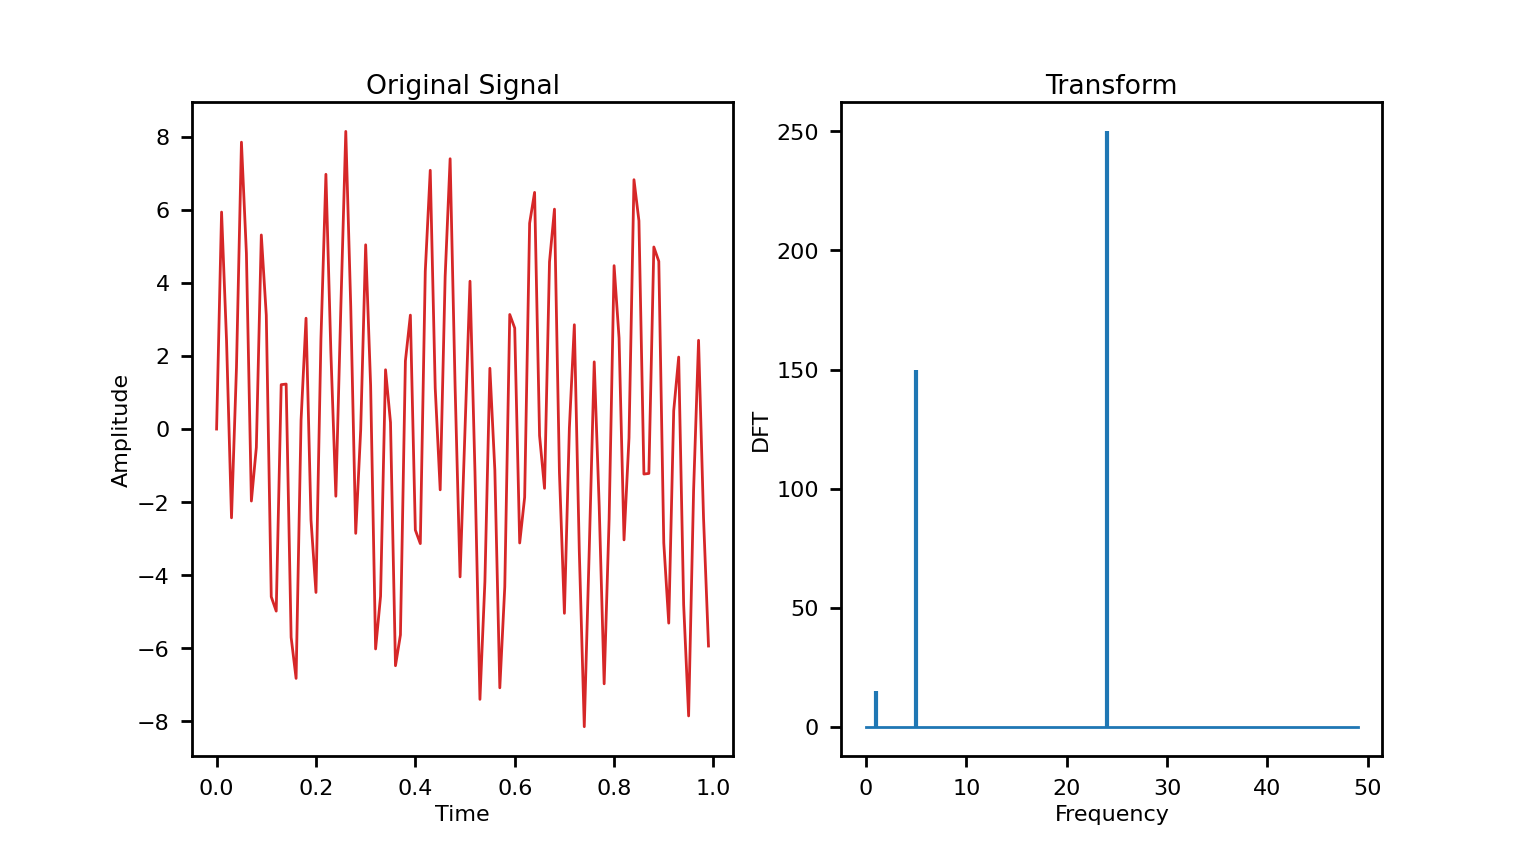
\includegraphics[width=1\linewidth]{figures/dft_example.png}
 %    \caption{DFT on $f(t) = 0.3\sin(2\pi t) + 5\sin(48 \pi t) + 3\sin(10 \pi t)$ with 100 equispaced sampling points}
 %    \label{fig:dft_ex}
 %\end{figure}

 
\subsubsection{Improving the DFT}
%Some transition statement here ...


 %Question 3.2.1
We consider a signal with a number of samples which is a power of two, that is, we restrict ourselves to \(N = 2^k, k \in \mathbb{Z^+}\). As a first step towards improving the performance of our DFT calculation, we will split the problem in two. Let \(n=N / 2\). By breaking \eqref{eq:dft} into sums over even and odd indices, we have
\begin{align}
    \begin{split}\label{eq:dft_split}
    \hat{f}_k &= \sum_{j=0}^{n-1} f_{2j} e^{\frac{-i2\pi k}{N}(2j)} + \sum_{j=0}^{n-1} f_{2j+1} e^{\frac{-i2\pi k}{N}(2j+1)} \\
    &= \sum_{j=0}^{n-1} f_{2j} e^{\frac{-i2\pi k}{N / 2}j} + e^{\frac{-i2\pi k}{N}} \sum_{j=0}^{n-1} f_{2j+1} e^{\frac{-i2\pi k}{N / 2}j} \\
    &= \sum_{j=0}^{n-1} f_{2j} \omega_n^{kj} + \omega_n^{k / 2} \sum_{j=0}^{n-1} f_{2j+1} \omega_n^{kj}.
    \end{split}
\end{align}

For \(k = 0, 1, \dots, n-1\), these two sums bear a resemblance to our original DFT: the sum over the even indices looks like a DFT of the even samples, while the sum over the odd indices looks like a DFT of the odd samples. However, we want to compute the coefficients for the entire range \(k = 0, 1, \dots, 2n-2\). Observe that from periodicity of the exponential, we have \begin{align*}
    \omega_n^{\frac{1}{2}n}  = e^{\frac{-i 2\pi (n / 2)}{n}} = e^{-i\pi} = -1\;\;\;\mathrm{and}\;\;\;\omega_n^{n} = e^{\frac{-i 2\pi n}{n}} = e^{-i 2\pi} = 1.
\end{align*} Thus, \begin{align}\label{eq:dft_split_2nd_half}
    \begin{split}
    \hat{f}_{k+n} &= \sum_{j=0}^{n-1} f_{2j} \omega_n^{(k+n)j} + \omega_n^{(k+n) / 2} \sum_{j=0}^{n-1} f_{2j+1} \omega_n^{(k+n)j} \\
    &= \sum_{j=0}^{n-1} f_{2j} \omega_n^{kj} \left(\omega_n^{n}\right)^j  + \omega_n^{k / 2} \omega_n^{n / 2} \sum_{j=0}^{n-1} f_{2j+1} \omega_n^{kj} \left(\omega_n^{n}\right)^j \\
    &= \sum_{j=0}^{n-1} f_{2j} \omega_n^{kj} - \omega_n^{k / 2}  \sum_{j=0}^{n-1} f_{2j+1} \omega_n^{kj}.
    \end{split}
\end{align}

Together, \eqref{eq:dft_split} and \eqref{eq:dft_split_2nd_half} allow us to compute the coefficients \(\hat{f}_k\) in terms of the DFT of the even sample terms and the DFT of the odd sample terms.

We rearrange our sample vector \(\vec{f}\) to place even indexed samples before odd indexed samples,
\begin{align*}
    \vec{f}^* = \begin{bmatrix}
        f_0 \\ f_2 \\ \vdots \\ f_{2n-2} \\ f_1 \\ f_3 \\ \vdots \\ f_{2n-1}
    \end{bmatrix} = \begin{bmatrix}
        \vec{f_{even}} \\ \vec{f_{odd}}
    \end{bmatrix}.
\end{align*} Our system now becomes \(\hat{\vec{f}} = F^* \vec{f}^*\), where \begin{align*}
    F^* = \begin{bmatrix}
        % lower half of coefficients (k <= n-1)
        1 & 1              & \dots & 1                   
            & 1                        & 1                              & \dots & 1 \\
        1 & \omega_n       & \dots & \omega_n^{n-1}      
            & \omega_n^{\frac{1}{2}}   & \omega_n^{\frac{1}{2}+1}       & \dots & w_n^{\frac{1}{2}+(n-1)} \\
        \vdots &           & \ddots & \vdots             
            & \vdots                   &                                & \ddots & \vdots \\
        1 & \omega_n^{n-1} & \dots  & \omega_n^{(n-1)^2}
            & \omega_n^{\frac{n-1}{2}} & \omega_n^{\frac{n-1}{2} + n-1} & \dots & \omega_n^{\frac{n-1}{2} + (n-1)^2} \\
        % upper half of coefficients (k >= n)
        1 & 1              & \dots & 1                   
            & -1                        & -1                              & \dots & -1 \\
        1 & \omega_n       & \dots & \omega_n^{n-1}      
            & -\omega_n^{\frac{1}{2}}   & -\omega_n^{\frac{1}{2}+1}       & \dots & -w_n^{\frac{1}{2}+(n-1)} \\
        \vdots &           & \ddots & \vdots             
            & \vdots                   &                                & \ddots & \vdots \\
        1 & \omega_n^{n-1} & \dots  & \omega_n^{(n-1)^2}
            & -\omega_n^{\frac{n-1}{2}} & -\omega_n^{\frac{n-1}{2} + n-1} & \dots & -\omega_n^{\frac{n-1}{2} + (n-1)^2} \\
    \end{bmatrix}.
\end{align*}

The top half of the \(F^*\) matrix is from \eqref{eq:dft_split} while the bottom half is from \eqref{eq:dft_split_2nd_half}. We can factor \(F^*\) as
\begin{align*}
    F^* = RG &=
    \begin{bmatrix}
        1 & 0 & \dots & 0 & 1 & 0 & \dots & 0 \\
        0 & 1 & \dots & 0 & 0 & \omega_n^{\frac{1}{2}} & \dots & 0 \\
        \vdots & & \ddots & & \vdots & & \ddots & \\
        0 & 0 & \dots & 1 & 0 & 0 & \dots & w_n^{\frac{n-1}{2}} \\
        1 & 0 & \dots & 0 & -1 & 0 & \dots & 0 \\
        0 & 1 & \dots & 0 & 0 & -\omega_n^{\frac{1}{2}} & \dots & 0 \\
        \vdots & & \ddots & & & \vdots & & \ddots & \\
        0 & 0 & \dots & 1 & 0 & 0 & \dots & -w_n^{\frac{n-1}{2}}
    \end{bmatrix} \begin{bmatrix}
        1 & 1 & \dots & 1 & 0 & 0 & \dots & 0 \\
        1 & \omega_n & \dots & \omega_n^n & 0 & 0 & \dots & 0 \\
        \vdots & & \ddots & \vdots & \vdots & & \ddots & \vdots \\
        1 & \omega_n^{n-1} & \dots & \omega_n^{(n-1)^2} & 0 & 0 & \dots & 0 \\
        0 & 0 & \dots & 0 & 1 & 1 & \dots & 1  \\
        0 & 0 & \dots & 0 & 1 & \omega_n & \dots & \omega_n^n  \\
        \vdots & & \ddots & \vdots & \vdots & & \ddots & \vdots \\
        0 & 0 & \dots & 0 & 1 & \omega_n^{n-1} & \dots & \omega_n^{(n-1)^2} \\
    \end{bmatrix} \\
    &= \begin{bmatrix}
        I_{n} & D_{n} \\
        I_{n} & -D_{n} \\
    \end{bmatrix} \begin{bmatrix}
        F_n & 0 \\
        0 & F_n \\
    \end{bmatrix},
\end{align*} where \(D_n\) is the diagonal matrix multiplied before the odd part of the DFT, \begin{align*}
    D_n = \begin{bmatrix}
        1 & 0 & 0 & \dots & 0 \\
        0 & \omega_n^{\frac{1}{2}} & 0 & \dots & 0 \\
        0 & 0 & \omega_n^{\frac{2}{2}} & \dots & 0 \\
        \vdots & & & \ddots & \\
        0 & 0 & 0 & \dots & \omega_n^{\frac{n-1}{2}}
    \end{bmatrix}.
\end{align*}

\tikzstyle{samp} = []
\tikzstyle{block_dft} = [rectangle, draw, fill=gray!20, text centered, inner sep=1em]
\tikzstyle{block} = [rectangle, draw, fill=white, text centered, inner sep=0.5em]
\tikzstyle{block_sum} = [circle, draw, fill=white, 
    text centered, inner sep=0.5em]
\tikzstyle{line} = [draw, -triangle 45]

\begin{figure}
    \centering
    \begin{tikzpicture}[node distance = 10em, x=12em, y=4em]
        \node [samp] at (-0.5, 6) (f0) {$f_0$};
        \node [samp] at (-0.5, 5) (f1) {$f_1$};
        \node [samp] at (-0.5, 4) (f2) {$f_2$};
        \node [samp] at (-0.5, 3) (f3) {$f_3$};
        \node [samp] at (-0.5, 2) (f_dots) {$\vdots$};
        \node [samp] at (-0.5, 1) (f2n2) {$f_{2n-2}$};
        \node [samp] at (-0.5, 0) (f2n1) {$f_{2n-1}$};

        \node [samp] at (0.5, 5) (feven) {$\begin{bmatrix}
            \\
            \vec{f_{even}} \\
            \\
        \end{bmatrix}$};
        \node [samp] at (0.5, 1) (fodd) {$\begin{bmatrix}
            \\
            \vec{f_{odd}} \\
            \\
        \end{bmatrix}$};

        \node [block_dft] at (1, 5) (dfteven) {DFT};
        \node [block_dft] at (1, 1) (dftodd) {DFT};

        \node [block] at (1.5, 1) (di) {$-D_n$};
        \node [block] at (1.35, 2.4) (d) {$D_n$};

        \node [block_sum] at (2, 1) (sumi) {$+$};
        \node [block_sum] at (2, 5) (sum) {$+$};

        \node [samp] at (2.5, 3) (fk) {$\begin{bmatrix}
            \\
            \;\;\vec{\hat{f}}\;\; \\
            \\
        \end{bmatrix}$};

        \path [line] (f0) -- (feven);
        \path [line] (f2) -- (feven);
        \path [line] (f2n2) -- (feven);
        \path [line] (f1) -- (fodd);
        \path [line] (f3) -- (fodd);
        \path [line] (f2n1) -- (fodd);

        \path [line] (feven) -- (dfteven);
        \path [line] (fodd) -- (dftodd);

        \path [line] (dftodd) -- (di);
        \path [line] (dftodd) -- (d);

        \path [line] (di) -- (sumi);
        \path [line] (d) -- (sum);
        \path [line] (dfteven) -- (sum);
        \path [line] (dfteven) -- (sumi);

        \path [line] (sum) -- (fk);
        \path [line] (sumi) -- (fk);
            
    \end{tikzpicture}
    \caption{A single step of computation for the FFT on samples \(f\). The input data is split into two components \(f_{even}\) and \(f_{odd}\), over which the DFT is computed. The DFT may be computed by recursive application of the FFT to \(f_{even}\) and \(f_{odd}\). The resulting coefficients \(\hat{f}\) are formed from a linear combination of the two DFT results.}
    \label{fig:fft_schematic}
\end{figure}

%\begin{figure}
%    \centering
%    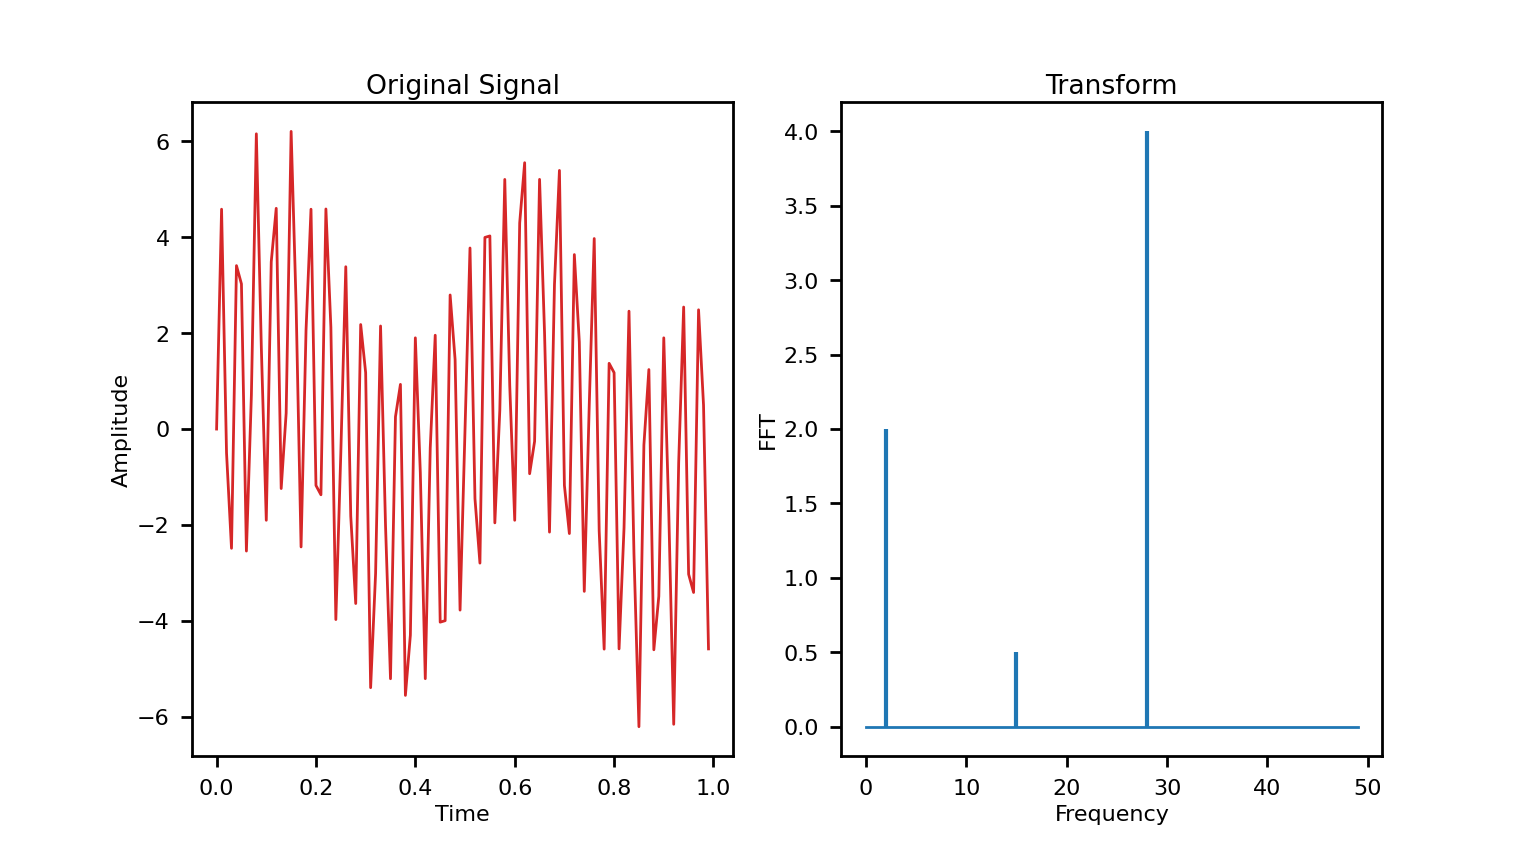
\includegraphics[width=1\linewidth]{figures/fft_ex.png}
%    \caption{FFT on $f(t) = 2\sin(4\pi t) + 4\sin(56 \pi t) + 0.5\sin(30 \pi t)$ with 100 equispaced sampling points}
%    \label{fig:enter-label}
%\end{figure}




The importance of this method simply cannot be understated. By exploiting this symmetry repeatedly, the time complexity is reduced
to $\mathcal{O}(n\log n)$.\\

To emphasize precisely how impactful this is on real world analysis, we tested an example signal of three superimposed sine waves on both the DFT and FFT for a number of points ranging from 1000 to 1000. Each interval was tested ten times, and the average is plotted. The results, shown in \ref{fig:timecomp} demonstrate how much time can be saved. 
%\begin{figure}
%     \centering
%     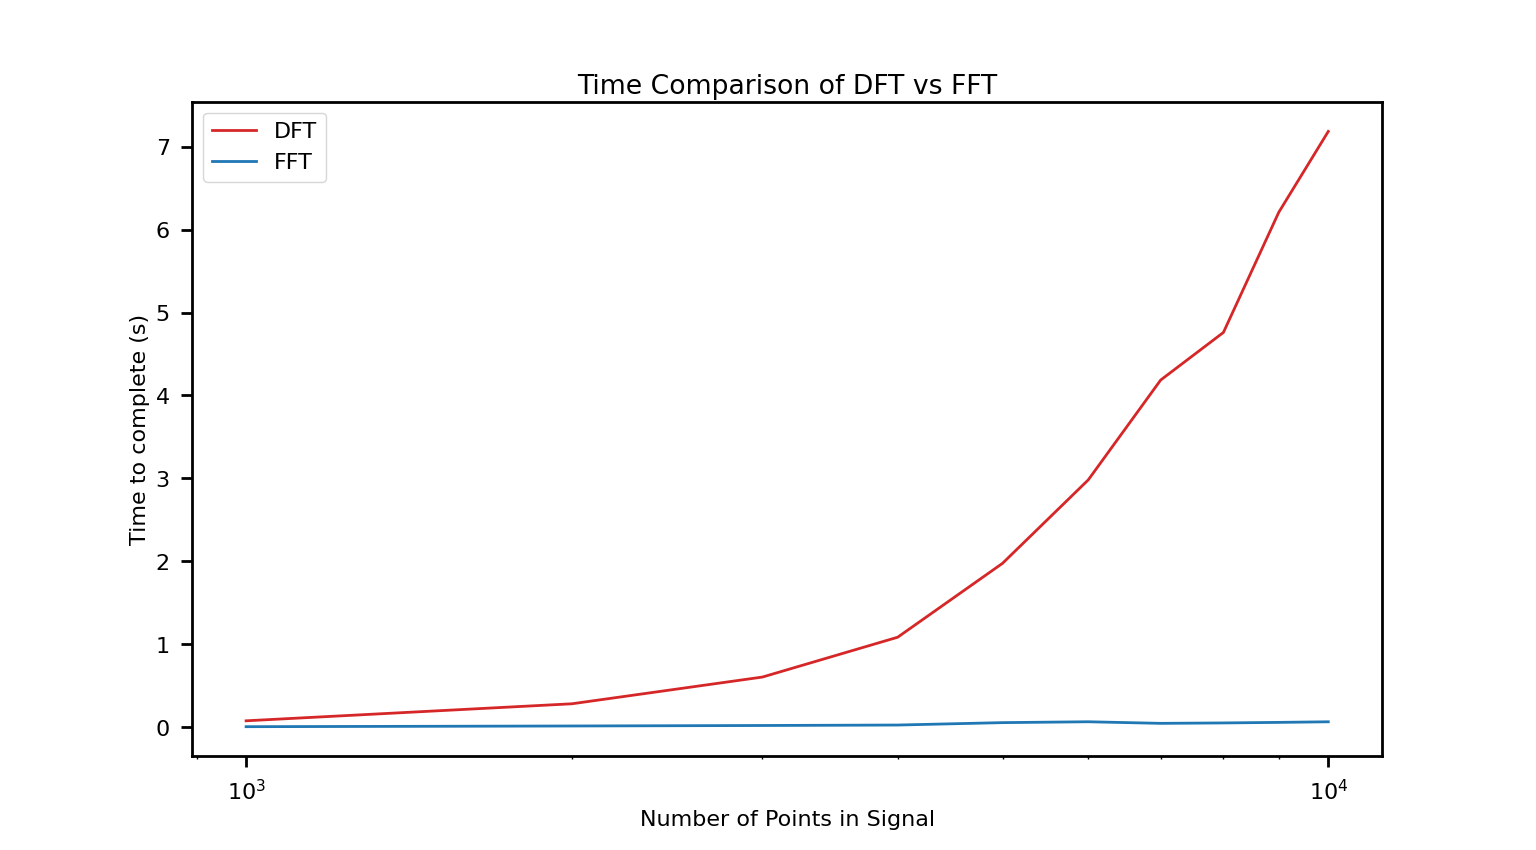
\includegraphics[width=1\linewidth]{figures/dft_fft_comp_nolog_big.png}
%     \caption{Computational time DFT and FFT analyzed with varying sample points}
%     \label{fig:timecomp}
%\end{figure}

 Further, in order for the FFT to take just as much time as the DFT processing a signal with 10,000 samples, the FFT must process a signal of roughly 1,000,000 samples. \\

Arguably just as paramount, the spatial complexity of the methods also contributes to the favorability of the fft. In order to create the matrix shown in ??? REF, we require the allocation of $n^2$ floating points in memory. As such, our machines struggle to process anything larger than 20,000 samples when computing the DFT. In contrast, the FFT can easily compute signals with millions of sample points without issue.\\

\section{Short-Time Fourier Transform}
Since many signals in the real world are time-dependent, the STFT is an invaluable tool for analyzing and understanding real-world data. The FFT exists only in the frequency domain, so it can provide no information as to a signal's behavior over time. Often, we desire to know information about the time domain of a signal, namely how that signal changes over a period. To do this, we explore the Short-Time Fourier Transform, which we derive and apply in the following section.\\
\subsection{Derivation}
\subsubsection{Continuous}
With continuous data $f$, we analyze a given section to determine behavior in the time domain. For some window function $g(x)$, we can perform the analysis with an integral, where 

\begin{equation}\label{continuous-stft}
    \int_\mathcal{D} f(t)\overline{g(t-x)}e^{-2\pi i \omega t} dt
\end{equation}.


Note the similarity to the standard Fourier transform, which takes the form \\
\begin{align*}
    &\int_\mathcal{D} f(t)e^{-2\pi i \omega t} dt
\end{align*}.
With this insight, we see more intuitively how the introduction of a window function introduces 
\subsubsection{Discrete}
Similar to section ??? we discretize this process by considering a finite number of points. As such, we have the resulting sum: \\
\begin{equation}\label{discrete-stft}
    \sum_{n=0}^{N-1}g(n)f(n+mH)e^{-i\frac{2\pi}{N}\omega n}
\end{equation}
\subsection{Application}


\noindent\makebox[\linewidth]{\rule{\paperwidth}{0.94pt}}

\section{Project Overview}

In this project, we investigate the Fast Fourier Transform (FFT), a method for trigonometric interpolation on equispaced points along an interval that uses symmetry to reduce computational complexity from $\mathcal{O}(n^2)$ to $\mathcal{O}(n\log n)$. We begin with a derivation of the Discrete Fourier Transform (DFT), then show its drawbacks, focusing on computational complexity, and propose the FFT as an alternative. We explore the properties of the FFT, including its restrictions on the sample points, and compare its performance to that of the DFT. We continue with an exploration of the Short-Time Fourier Transform (STFT), a common tool in signal analysis and processing.

\section{Introductory Material}

\subsection{Introduction}
We introduce the Fourier transform as a tool for understanding the spectral content of a signal and show how the transform is useful in a wide variety of applications. We motivate the desire to apply the transform over sampled signals with a finite number of points.

\subsection{Discrete Fourier Transform (DFT)}

We introduce the Fourier series representations of periodic signals and its extension to the Fourier transform on aperiodic signals. We show how discrete signals over a finite time interval can be represented by a truncated Fourier series, and introduce the discrete Fourier transform (DFT) as a means to compute such a representation \cite{oppenheim1997signals}. We show how the DFT can be computed through the solution to a linear system in $\mathcal{O}(n^2)$ time complexity. We demonstrate the relationships between Fourier series representations in complex exponential and real forms and show how to convert between the two.

\subsection{Fast Fourier Transform (FFT)}
We then demonstrate a method to overcome $\mathcal{O}(n^2)$ complexity and reduce to $\mathcal{O}(n\log(n))$ time. We restrict ourselves to discrete signals with a number of points that are an integer power of 2 and rearrange the signal into odd and even data points. From here, we derive a matrix factorization that exploits sparsity and show how the structure of the matrix allows us to continually divide the signal and save computations via symmetries.   

\section{Extension: Short-Time Fourier Transform}

\subsection{Introduction}

For our independent extension, we explore the Short-Time Fourier Transform (STFT), a method for analyzing signals with time-varying spectra. \cite{allen_mills_2004_signal_analysis} Since many signals in the real world are time-dependent, the STFT is an invaluable tool for analyzing and understanding real-world data; furthermore, the STFT leads to useful data visualization methods, such as spectrograms and waterfall plots, which we will also investigate.

\subsection{Derivation} We introduce the mathematical methods used to derive the STFT. We explore both the continuous\cite{Gröchenig2001} and discrete\cite{STFT-presentation} variants, focusing on the discrete variant, its parallels with the DFT, and its applications. After introducing several different windowing functions and analyzing their advantages and shortcomings, we motivate their use for specific scenarios; we also discuss the other input parameters to the STFT algorithm, such as window size, window overlap, and number of FFT points.

\subsection{Application} We demonstrate the applicability of the STFT by analyzing several example signals using the different methods explored in the previous section. We conclude with examples of visualizations and discussion of how these tools have contributed to various fields of science.
We use magnetometer data from the EMFISIS instrument suite aboard the Van Allen Probes to demonstrate the utility of the STFT in visualizing charged particle events in the Earth's magnetosphere. \cite{kletzing_et_al_2012_EMFISIS}

\section{Timeline and Work Distribution}

Our proposed timeline for the project is given below in Table \ref{tab:timeline}.

\begin{table}[H]
    \centering
    \begin{tabular}{|c|c|c|} 
     \hline
     Date range & Proposed work & Lead \\
     \hline
     Oct 24 - Nov 1 & Work on project proposal & Everyone \\
     \hline
     Oct 24 - Nov 8 & Research, find sources & Everyone \\
     \hline
     \textbf{Nov 1} & \textbf{Project proposal due} & Everyone \\ \hline
     Nov 1 - Nov 8 & Work on theoretical foundations (Sec 2.1 - 2.3, Start 3.1) & Elizabeth\\
     \hline
     Nov 8 - Nov 15 & Work more on 3.1 - 3.3& Edward\\
     \hline
     Nov 8 - Nov 15 & Write scripts for computing FFT/STFT and visuals & Erick\\
     \hline
     Nov 15 - Nov 22 & Finish rough draft & Everyone\\
     \hline
     \textbf{Nov 22} & \textbf{Project rough draft due} & Everyone \\ \hline
     Nov 22 - Nov 29 & Minor edits over break, clean up figures while waiting for feedback & Everyone \\
     \hline
     Nov 29 - Dec 6 & When we get feedback, meet and discuss revisions \& next steps & Everyone \\
     \hline
     Nov 29 - Dec 6 & Finish sections not fully in rough draft, extend where possible & Everyone\\
     \hline
    Dec 7 - Dec 15 & Improve Sec 2 & Erick \\ 
     \hline
     Dec 7 - Dec 15 & Improve Sec 3 & Elizabeth \\
     \hline
     Dec 7 - Dec 15 & Improve Formatting \& Visuals & Edward \\
     \hline
     \textbf{Dec 15} & \textbf{Project final draft due} & Everyone \\ \hline
    \end{tabular}
    \caption{Proposed project timeline.}
    \label{tab:timeline}
\end{table}

\printbibliography

\end{document}
